\documentclass[12pt,letterpaper]{article}
\usepackage[margin=1in]{geometry}
\usepackage{fancyhdr}
\usepackage[utf8]{inputenc}
\usepackage{palatino}
\usepackage{microtype}
\usepackage{hyperref}
\usepackage{graphicx}
\usepackage{lastpage}
\usepackage[hang,small,margin=1in]{caption}
\usepackage{titlesec}

\renewcommand{\headrulewidth}{0pt}
\fancyfoot{}
\fancyfoot[C]{\sffamily Page \thepage\ of \pageref{LastPage}}
\pagestyle{fancy}

\titleformat{\section}{\bfseries\MakeUppercase}{\arabic{\thesection}}{1em}{}
\titleformat{\subsection}{\bfseries}{\arabic{\thesection}.\arabic{\thesubsection}}{1em}{}
\titleformat{\subsubsection}{\itshape}{\arabic{\thesection}.\arabic{\thesubsection}.\arabic{\thesubsubsection}}{1em}{}

\setlength{\parindent}{0cm}
\setlength{\parskip}{1em}

\captionsetup[figure]{labelfont=it, font=it}
\captionsetup[table]{labelfont={it,sc}, font={it,sc}}

\hypersetup{colorlinks, linkcolor = black, citecolor = black, urlcolor = black}
\urlstyle{same}



\begin{document}

\fancyfoot{}
\begin{center}
    \hfill \\
    \vspace{4in}
    {\bf\Huge CS457 Project \#6 \\}
    \vspace{2in}
    {\Large Soo-Hyun Yoo \\ February 18, 2015}
\end{center}

\newpage
\fancyfoot[C]{\sffamily Page \thepage\ of \pageref{LastPage}}

\section*{Source Files}

\begin{itemize}
    \item p6.glib
    \item p6.vert
    \item p6.frag
\end{itemize}


\section*{Explanation}

\subsection*{p6.glib}

We put ourselves in orthographic mode, place the eye at positive Z, and point
the camera at the origin with positive Y as the up vector.

We load the input image as a {\tt Texture2D} and declare the vertex and
fragment files to be used as well as some variables to display in sliders and
checkboxes.

\subsection*{p6.vert}

The vertex file in this project simply outputs the ST coordinates for the
fragment shader.

\subsection*{p6.frag}

We declare the input vectors and uniform variables.

We define {\tt isInside}, a convenience function to determine whether or not
a given set of ST coordinates is inside a rectangle or circle (the lens) of the
user-specified dimension and location.

In {\tt main}, if the ST position is deemed inside the lens, we grab a pixel
a distance scaled away from and rotated about the lens center. The color here
is then updated before being sharpened.


\newpage
\section*{Results}

\begin{figure}[!h]
    \centering
    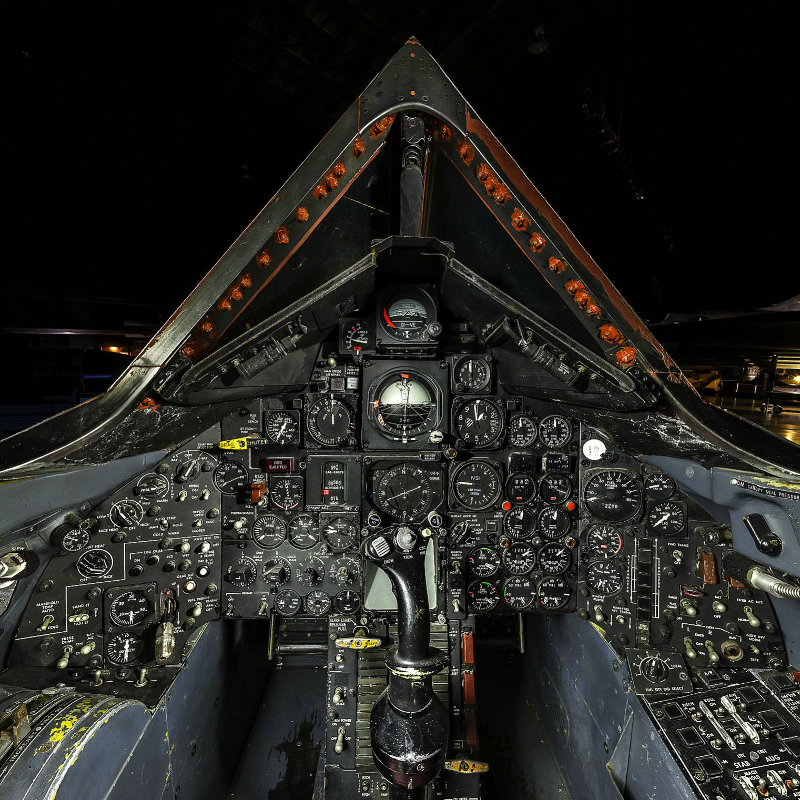
\includegraphics[width=1.0\textwidth]{img/sr71.png}
    \caption{Original input image, the SR-71 cockpit.}
\end{figure}

\begin{figure}[!h]
    \centering
    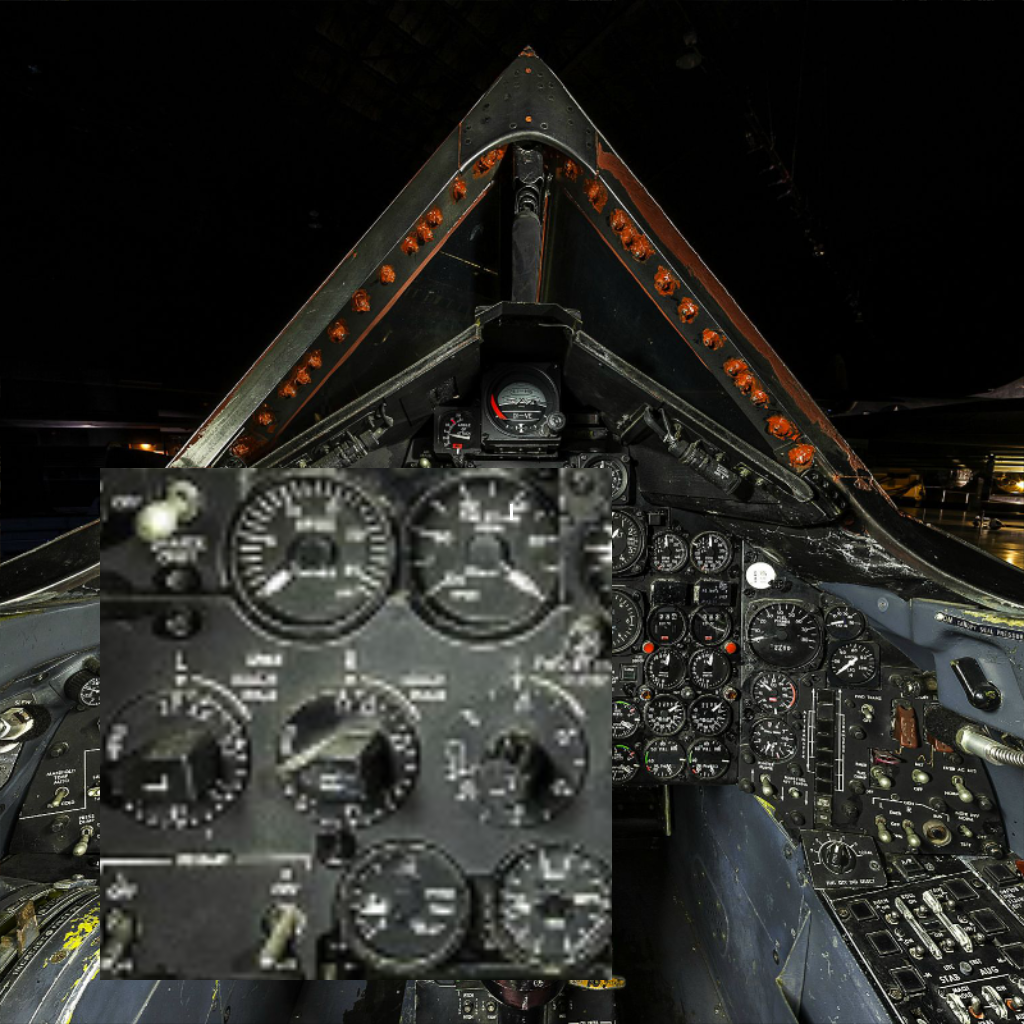
\includegraphics[width=1.0\textwidth]{img/mag.png}
    \caption{Magnified}
\end{figure}

\begin{figure}[!h]
    \centering
    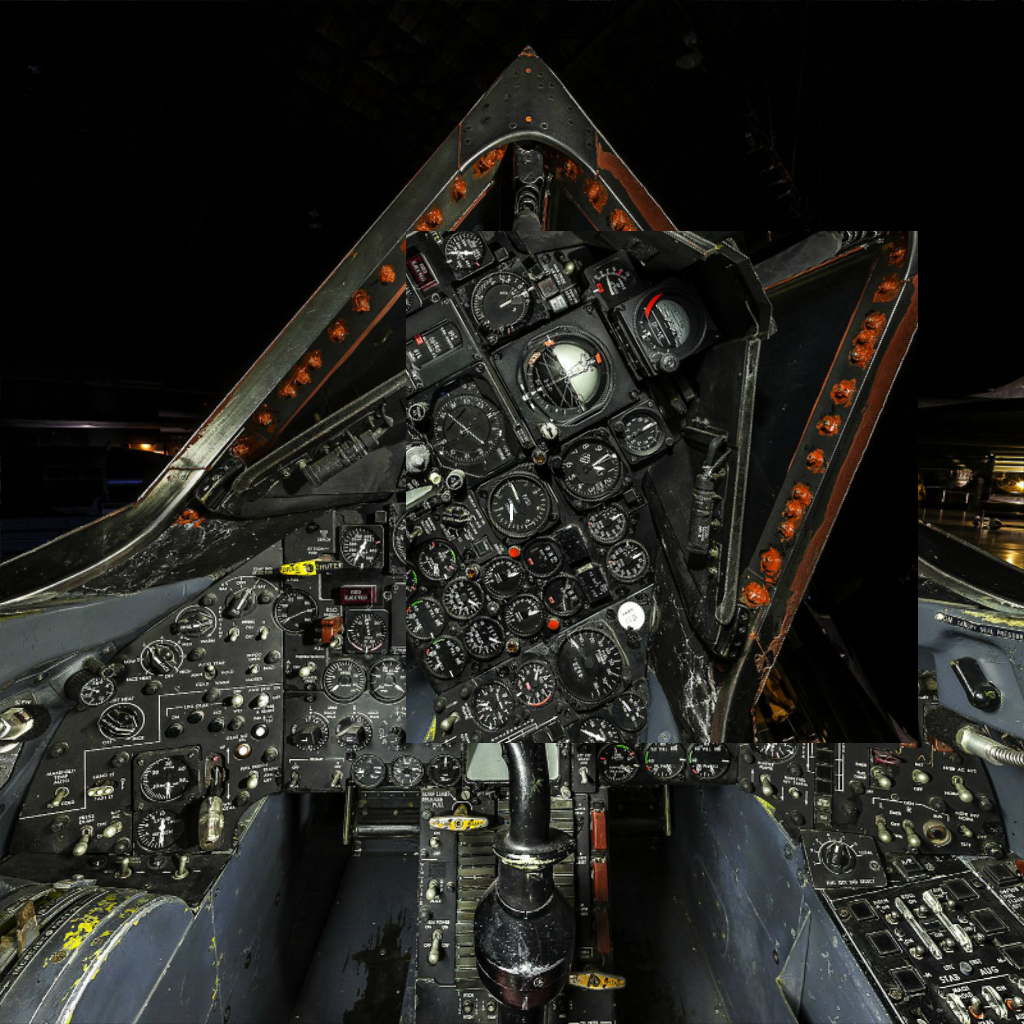
\includegraphics[width=1.0\textwidth]{img/rot.png}
    \caption{Rotated}
\end{figure}

\begin{figure}[!h]
    \centering
    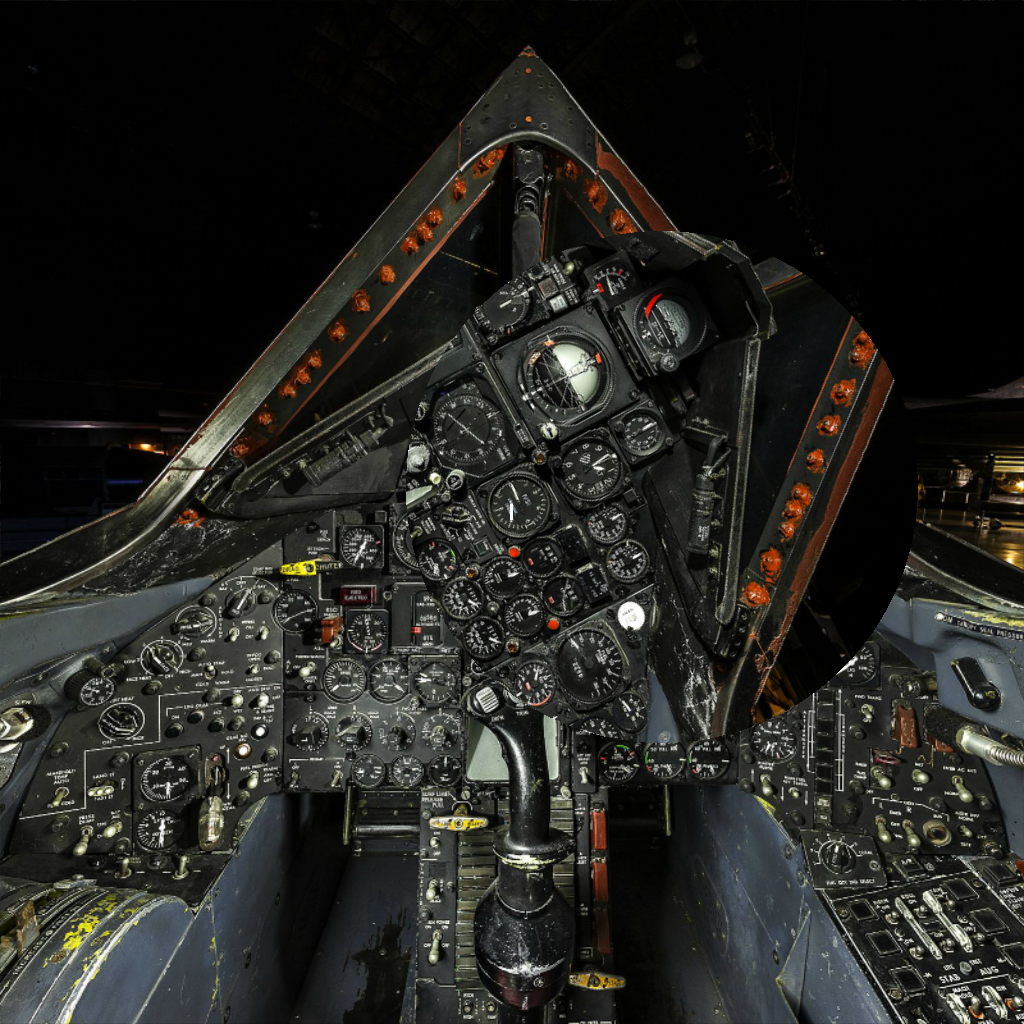
\includegraphics[width=1.0\textwidth]{img/circlerot.png}
    \caption{Rotated with circular lens}
\end{figure}

\begin{figure}[!h]
    \centering
    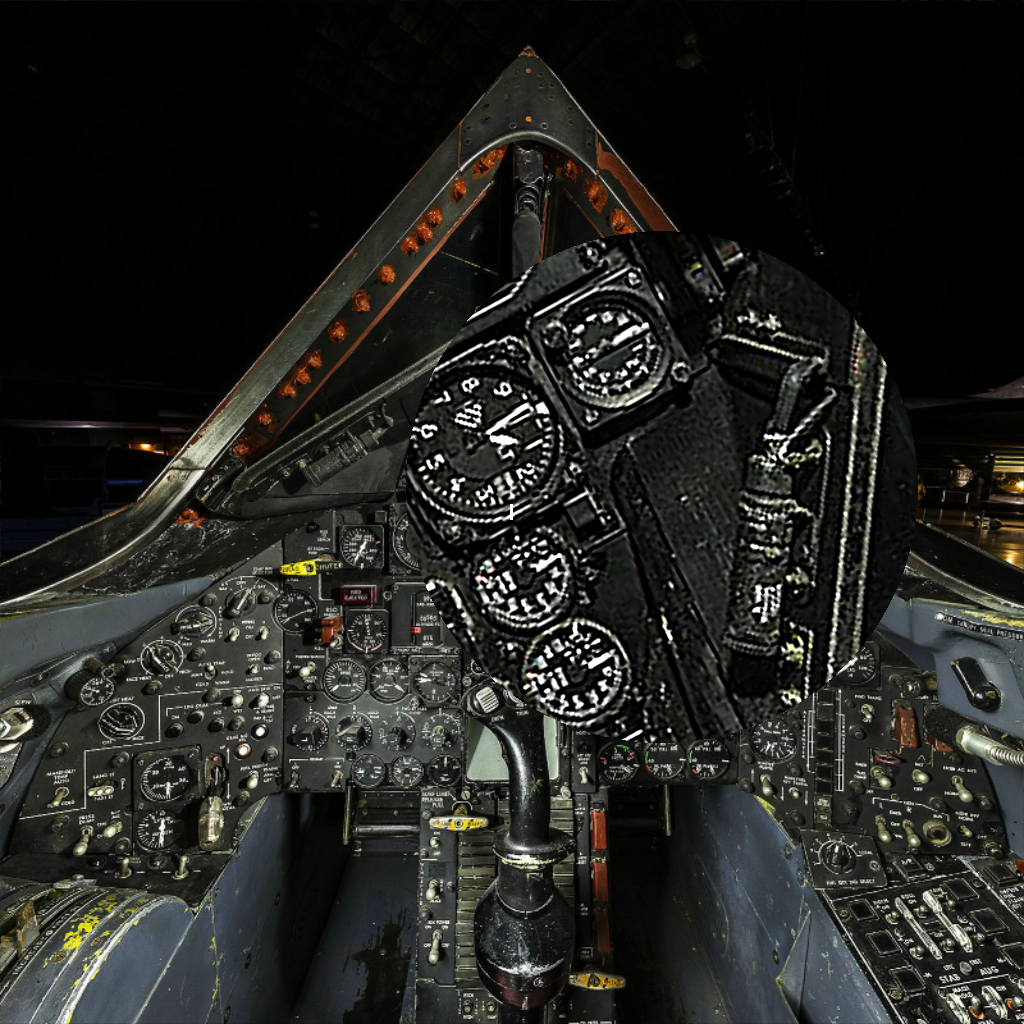
\includegraphics[width=1.0\textwidth]{img/sharp.png}
    \caption{Sharpened}
\end{figure}

\begin{figure}[!h]
    \centering
    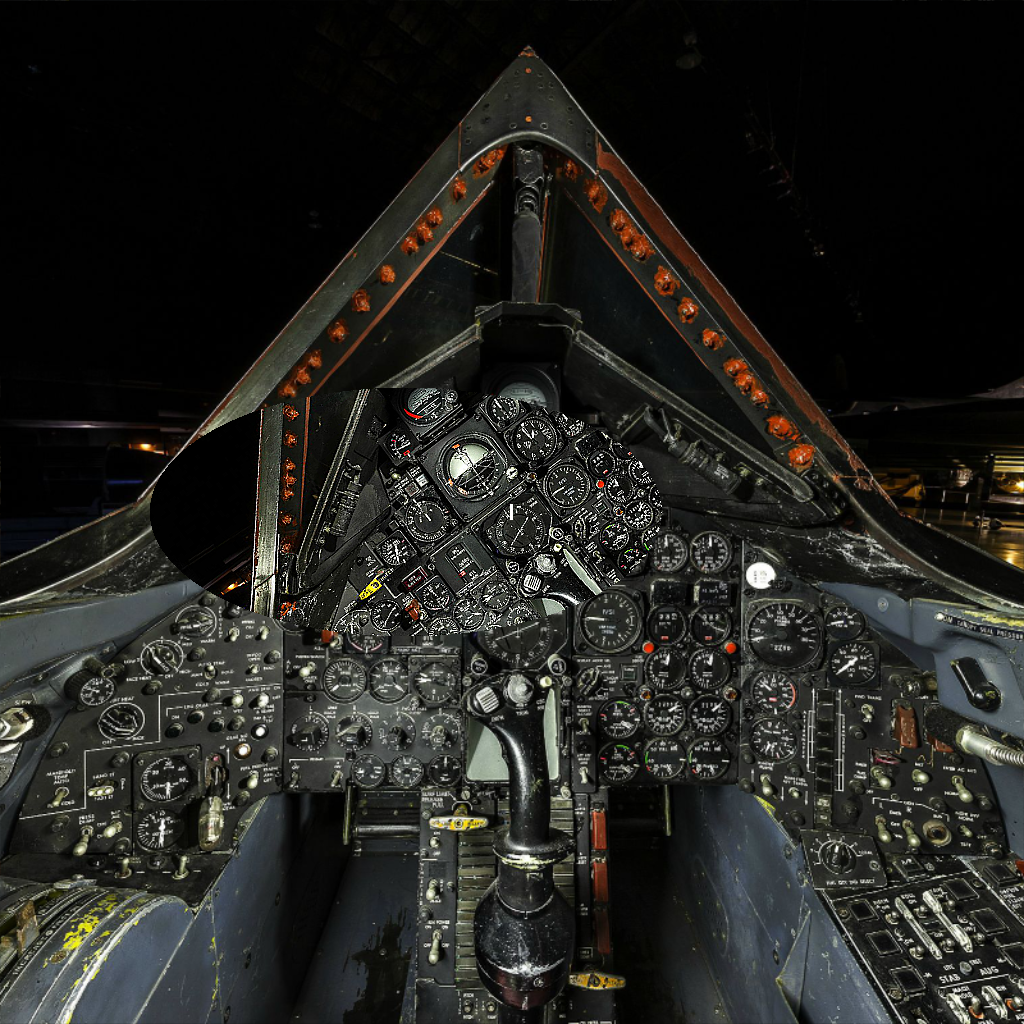
\includegraphics[width=1.0\textwidth]{img/asymmetric.png}
    \caption{Asymmetric lens}
\end{figure}

\end{document}
